\documentclass[12pt,oneside,a4paper]{estilo}

% --- Pacotes adicionais estritamente de conteúdo ---
\usepackage{tabularx}
\usepackage{float} 
\usepackage{booktabs}
\usepackage{graphicx}
\usepackage{amsmath, amsfonts, amssymb}
\usepackage{booktabs}
\usepackage{microtype}          
\usepackage{hyperref}
\hypersetup{
  colorlinks=true,
  linkcolor=blue,
  citecolor=blue,
  urlcolor=blue,
  pdftitle={Pipeline RAG para o SEEU},
  pdfauthor={Gabriel Oliveira Faria, Pedro Samuel, Zandor Duarte},
}

% --- Se o estilo NÃO carregar abntex2cite ---
\usepackage{abntex2cite}

\begin{document}

% ====================================================
% Elementos pré-textuais
% ====================================================
\pretextual
\begin{center}
{\ABNTEXchapterfont\large CENTRO UNIVERSITÁRIO DO DISTRITO FEDERAL -- UDF}\\
\vspace{2cm}
{\ABNTEXchapterfont\Large Gabriel Oliveira Faria\\Pedro Samuel\\Zandor Duarte}
\vspace{3cm}
{\ABNTEXchapterfont\Large Pipeline RAG para o SEEU: Modernização da Execução Penal com IA e Busca Vetorial}
\vspace{6cm}
\end{center}
\begin{flushright}
Brasília\\
2024
\end{flushright}

%
% Documento: FOLHA DE ROSTO
%

\makeatletter
\begin{folhaderosto}
	\thispagestyle{empty}%limpa estilo da pagina
	
    \begin{center}
    
		\small\textbf{\expandafter\uppercase\expandafter{\imprimirnomeautor}}\\
		\vspace*{5.2 cm}%Espaço entre linhas
		\normalsize\textbf{\expandafter\uppercase\expandafter{\imprimirtitulotb}}\\
		
    \end{center}
	
	\vspace*{2.35 cm}%Espaçamento entre linhas
		    \large%tamanho da fonte 
    		\hfill%Estica horizontamente  com espaços
	    	\begin{minipage}{8 cm}%Minipagina
	    		\begin{small} %Muda tamanho da fonte
	    		\setlength{\baselineskip}{0.8\baselineskip}
				
				
		    	{Dissertação apresentada junto ao programa de {\textbf{\imprimirprograma}}
		    	do {\textbf{\imprimirinstituicao}},
		    	como requisito parcial à obtenção do título de
		    	{\textbf{\imprimirgrau}}.}\\{
		    	}\\\textbf{Orientadora}:\\ \\
		    	{\imprimirtitulacaoorientador }{ }{\imprimirorientador.}\\{
		    	}\\\textbf{Coorientador}:\\ \\ {\imprimirtitulacaocoorientador }{ }{\imprimircoorientador.}
				
				
				\end{small} %Muda tamanho da fonte
		    \end{minipage}%%Minipagina
		    	
		    \vspace*{6.5 cm}%Espaçamento entre linhas
		    
		    \begin{center} %Alinhamento centralizado
		    	\normalsize %Muda tamanho da fonte
	    		\textbf{\imprimirlocalapresentacao, \imprimirdataapresentacao}
	    	\end{center}%Alinhamento centralizado

\end{folhaderosto}
\makeatother

%
% Documento: FOLHA APROVAÇÃO
%

\makeatletter
\begin{folhadeaprovacao}
	
	\thispagestyle{empty}%limpa estilo da pagina
	
	\begin{center}
		
		\small\textbf{\expandafter\uppercase\expandafter{\imprimirnomeautor}}\\
		\vspace*{3.0 cm}%Espaço entre linhas
		\normalsize\textbf{\expandafter\uppercase\expandafter{\imprimirtitulotb}}
		
	\end{center}
	
	\vspace*{0.35 cm}%Espaçamento entre linhas
	\large%tamanho da fonte 
	\hfill%Estica horizontamente  com espaços
	\begin{minipage}{10 cm}%Minipagina
		\begin{small} %Muda tamanho da fonte
			\setlength{\baselineskip}{\baselineskip}
			
			
			{Monografia apresentada ao programa de {\textbf{\imprimirprograma}}
				do {\textbf{\imprimirinstituicao}},
				como requisito à obtenção do título de
				{\textbf{\imprimirgrau}}.}\\
			
			{\textbf{Data de aprovação:}\\
				18/12/2019
			}
			\vspace*{1.0 cm}
		
			{\textbf{Banca Examinadora:}\\
				
				\vspace*{1.0 cm}
				
				\rule{\linewidth}{.1 mm}\\
				{\textbf{Prof. Me. Diogo Dantas Moreira}\\
					Instituição de Ensino
				}
			
				\vspace*{1.0 cm}

				\rule{\linewidth}{.1 mm}\\
				{\textbf{Prof. Fulano}\\
					Instituição de Ensino
				}
			
				\vspace*{1.0 cm}
				
				\rule{\linewidth}{.1 mm}\\
				{\textbf{Prof. Fulano}\\
					Instituição de
				Instituição de Ensino}
			}
			
			
		\end{small} %Muda tamanho da fonte
	\end{minipage}%%Minipagina
	
	\vspace*{0.6 cm}%Espaçamento entre linhas
	
	\large%%tamanho da fonte 
	\hfill%%Estica horizontamente  com espaços
	
	
	\normalsize %Muda tamanho da fonte
	\vspace*{1.5 cm}%Espaçamento entre linhas
	
%	\begin{flushleft}%Alinhamento centralizado
%		%\textbf{Banca Examinadora}\\ %Negrito
%		
%		\vspace*{2 cm}%Espaçamento entre linhas
%		\rule{12 cm}{.1 mm}\\
%		{\imprimirtitulacaoorientador}{ }{\imprimirorientador} - Orientador\\
%		
%		\vspace*{1 cm}%Espaçamento entre linhas
%		\rule{12 cm}{.1 mm}\\
%		{\imprimirtitulacaocoorientador}{ }{\imprimircoorientador} - Coorientador\\
%		
%		
%		\imprimirtitulacaoexamum\imprimirnmexamum{} - \imprimirinstexamum /\imprimirdepartamentoexamum
%		
%		\vspace*{1 cm}%Espaçamento entre linhas
%		
%		
%		\vspace*{1.3 cm}%Espaçamento entre linhas
%	\end{flushleft}%Alinhamento centralizado
%	
	
\end{folhadeaprovacao}
\makeatother
%
% Documento: Dedicatória
%

\thispagestyle{empty}
\begin{dedicatoria}

Dedicação
\end{dedicatoria}
%
% Documento: Agradecimento
%

\begin{agradecimento}
    \noindent Agradeço, primeiramente a Deus, por mais uma conquista; ao meu orientador, pela dedicação e correções

    \noindent \textbf{}
\end{agradecimento}



%
% Documento: Epígrafe
%
\thispagestyle{empty}
\begin{epigrafe}
\begin{em}
``bob marley phrase''
\newline
\newline
\end{em}
\begin{autorepigrafe}
\textbf{Siddhartha Gautama}, Dhammapada
\end{autorepigrafe}

\end{epigrafe}



%
% Documento: Resumo (Português)
%

\begin{RESUMO}
\thispagestyle{empty}
\OnehalfSpacing

\noindent Este Trabalho de Conclusão de Curso apresenta o desenvolvimento de uma pipeline de Geração de Respostas Aumentada por Recuperação de Informação — Retrieval Augmented Generation (RAG ) aplicada ao Sistema Eletrônico de Execução Unificado (SEEU), do Conselho Nacional de Justiça (CNJ). O objetivo é melhorar a obtenção de dados de suporte do SEEU. Facilitando o uso pelos diferentes perfis de usuário da plataforma, integrando bancos de dados vetoriais a um Large Language Model (LLM), de modo a fornecer respostas em linguagem natural fundamentadas em documentos originais. A metodologia abrange a coleta automatizada de documentos oficiais em PDF; o pré-processamento com limpeza e segmentação textual; a vetorização por embeddings e indexação em mecanismo de busca semântica; a orquestração, por meio da biblioteca LangChain, entre o motor de recuperação FAISS ou OpenSearch e o LLM; e a disponibilização do serviço por chatbot e API REST. A avaliação empregará as métricas precisão, recall  e F1 score, bem como ensaios de usabilidade. Pretende-se reduzir em o 80\% o de busca e limitar a taxa de alucinação a cinco por cento. Os resultados esperados incluem ganho de eficiência na recuperação de informações, melhoria da qualidade das respostas e alinhamento às iniciativas Justiça 4.0 e o Objetivo de Desenvolvimento Sustentável (ODS 16), fortalecendo a transparência e o acesso à Justiça. Conclui-se que a arquitetura proposta viabiliza a transformação digital da execução penal e constitui base para expansões futuras no âmbito do Poder Judiciário.

\SingleSpacing
\noindent \textbf{Palavras-chaves}: execução penal; bancos de dados vetoriais; transformação digital.

\end{RESUMO}


%
% Documento: Resumo (Inglês)
%

\begin{ABSTRACT}
\thispagestyle{empty}
\OnehalfSpacing

\noindent This Final Undergraduate Thesis presents the development of a Retrieval Augmented Generation RAG pipeline applied to the Unified Electronic Penal Execution System SEEU of the National Council of Justice Its objective is to enhance data support retrieval within SEEU by facilitating use by different user profiles on the platform integrating vector databases with a Large Language Model LLM to provide naturallanguage responses grounded in original documents The methodology includes automated collection of official PDF documents preprocessing with cleaning and text segmentation embeddingbased vectorization and indexing in a semantic search engine orchestration via the LangChain library between the FAISS or OpenSearch retrieval engine and the LLM and deployment of the service via chatbot and REST API Evaluation will employ precision recall and F1 score metrics as well as usability testing The aim is to achieve an eighty percent reduction in search time and limit the hallucination rate to five percent Expected outcomes include improved information retrieval efficiency enhanced response quality and alignment with the Justice 40 initiative and UN SDG 16 strengthening transparency and access to justice It is concluded that the proposed architecture enables the digital transformation of penal execution and provides a foundation for future expansions within the Judiciary

\SingleSpacing
\noindent \textbf{Keywords}: penal execution; vector databases; digital transformation.

\end{ABSTRACT}

%-----------------------------------------------------------------
% LISTA DE ABREVIATURAS E SIGLAS
%-----------------------------------------------------------------
\begin{siglas}
  \item[API] \textit{Application Programming Interface}
  \item[CI/CD] \textit{Continuous Integration} / \textit{Continuous Deployment}
  \item[CKAN] \textit{Comprehensive Knowledge Archive Network}
  \item[CNJ] Conselho Nacional de Justiça
  \item[DPR] \textit{Dense Passage Retrieval}
  \item[FAISS] \textit{Facebook AI Similarity Search}
  \item[IA] Inteligência Artificial
  \item[LEP] Lei de Execução Penal
  \item[LLM] \textit{Large Language Model}
  \item[ML] \textit{Machine Learning}
  \item[NLP] \textit{Natural Language Processing}
  \item[OCR] \textit{Optical Character Recognition}
  \item[ODS] Objetivos de Desenvolvimento Sustentável
  \item[ONU] Organização das Nações Unidas
  \item[PDF] \textit{Portable Document Format}
  \item[PNUD] Programa das Nações Unidas para o Desenvolvimento
  \item[RAG] \textit{Retrieval-Augmented Generation}
  \item[REST] \textit{Representational State Transfer}
  \item[SEEU] Sistema Eletrônico de Execução Unificado
  \item[SQL] \textit{Structured Query Language}
  \item[STJ] Superior Tribunal de Justiça
  \item[TJ-BA] Tribunal de Justiça da Bahia
  \item[TJ-CE] Tribunal de Justiça do Ceará
\end{siglas}
 

% ----- Sumário (limite até subseção) -----------------
\setcounter{tocdepth}{2} % 0=cap, 1=sec, 2=subsec
\sumario

% ====================================================
% Elementos textuais
% ====================================================
\textual
%%%%%%%%%%%%%%%%%%%%%%%%%%%%%%%%%%%%%%%%%%%%%%%%%%%%%%%%%%%%%%%%%%%%%%%%%%%%%%%
% CAPÍTULO 1 – INTRODUÇÃO
%%%%%%%%%%%%%%%%%%%%%%%%%%%%%%%%%%%%%%%%%%%%%%%%%%%%%%%%%%%%%%%%%%%%%%%%%%%%%%%

\chapter{Introdução}
\label{sec:introducao}

Em nível estadual, o Tribunal de Justiça da Bahia (TJ-BA) mantém cerca de
24\,000 execuções penais ativas no Sistema Eletrônico de Execução Unificado
(SEEU). Como a Lei de Execução Penal (LEP) impõe revisão trimestral e a
Súmula 533 do Superior Tribunal de Justiça (STJ) confirma esse prazo, são
necessários aproximadamente 8\,000 despachos por mês (267/dia)
\cite{brasil1984lep,stj2015sumula533}. No Mutirão Processual Penal 2024 foram
lançados 18\,600 atos em 60 dias, volume acima da meta da Portaria 304/2024 do
Conselho Nacional de Justiça (CNJ), o que evidencia sobrecarga
\cite{tjba2024mutirao,cnj2024portaria304}.

Situação semelhante ocorreu no Tribunal de Justiça do Ceará (TJ-CE): a elaboração
manual de 146 despachos consumiria mais de quatro horas, enquanto um robô
executa cada um em 30 s \cite{tjce2023robos}.  Esses dados reforçam a
pertinência da \emph{pipeline} de \emph{Retrieval-Augmented Generation} (RAG)
proposta, capaz de automatizar a busca semântica e gerar minutas, recuperando
produtividade sem prejudicar a qualidade nem as garantias processuais.

A digitalização dos serviços públicos tornou-se pilar da modernização judicial,
impulsionada por parcerias entre organismos internacionais e o Judiciário.  O
Programa das Nações Unidas para o Desenvolvimento (PNUD) e o CNJ, por exemplo,
firmaram projetos que ampliam a transparência e o acesso à Justiça por meio de
soluções digitais e governança inovadora \cite{undp2025pnudcnj}.

A experiência do \emph{e-Government} da Estônia mostra o impacto de
infraestrutura digital robusta: 98 \% das declarações de imposto passam a ser
enviadas on-line em poucos minutos, e o mesmo percentual de empresas é
registrado eletronicamente, aumentando a rastreabilidade e reduzindo fraudes
\cite{divald2021eformalization}. Guardadas as proporções, o SEEU enfrenta
desafio semelhante — consolidar milhares de atos processuais dispersos e
assegurar as revisões trimestrais obrigatórias. O caso estoniano indica que
automação e padronização digitais podem gerar ganhos análogos de eficiência e
transparência, reforçando o valor da \emph{pipeline} RAG proposta.

Apesar dos avanços, a consulta manual a grandes acervos documentais ainda é
demorada e sujeita a erros. Pesquisas mostram que bancos de dados vetoriais e
\emph{embeddings} reduzem a latência e aumentam a precisão de recuperação
\cite{taipalus2024vector,gao2023survey}. Técnicas RAG — que combinam
Inteligência Artificial (IA) e \emph{Large Language Models} (LLMs) — despontam
como solução para consultas em linguagem natural. Revisões recentes destacam o
potencial dessa abordagem \cite{qwak2024integrating,pujiono2024implementing}.

Este trabalho propõe construir uma \emph{pipeline} RAG para o SEEU,
implementada em Python, orquestrada por LangChain, exposta por chatbot em Flask
e empacotada em Docker para implantação consistente. Operadores do Direito
poderão realizar buscas intuitivas e integrar a solução a sistemas externos por
meio de uma Application Programming Interface (API) Representational State Transfer (REST).




%%%%%%%%%%%%%%%%%%%%%%%%%%%%%%%%%%%%%%%%%%%%%%%%%%%%%%%%%%%%%%%%%%%%%%%%%%%%%%%
% Seção 1.1 – Objetivos
%%%%%%%%%%%%%%%%%%%%%%%%%%%%%%%%%%%%%%%%%%%%%%%%%%%%%%%%%%%%%%%%%%%%%%%%%%%%%%%

\section{Objetivos}
\label{sec:objetivos}

\subsection{Objetivo Geral}
Desenvolver, para o SEEU, uma \emph{pipeline} RAG que automatize a recuperação
e a disponibilização de dados públicos da execução penal, oferecendo chatbot e
API REST, a fim de modernizar os processos judiciais e ampliar eficiência e
transparência.

\subsection{Objetivos específicos}
\begin{enumerate}[label=\arabic*.]
  \item Coletar e organizar os dados públicos do SEEU;
  \item Vetorizar esses dados em um banco vetorial (Elasticsearch, OpenSearch
        ou PostgreSQL + pgvector);
  \item Conectar o índice vetorial ao LLM selecionado;
  \item Testar a eficiência e a qualidade das respostas;
  \item Disponibilizar um chatbot integrado à \emph{pipeline};
  \item Conduzir testes de usabilidade e ajustar a experiência do usuário;
  \item Implementar uma API REST documentada;
  \item Preparar o ambiente de \emph{deployment} com segurança e escalabilidade.
\end{enumerate}

%%%%%%%%%%%%%%%%%%%%%%%%%%%%%%%%%%%%%%%%%%%%%%%%%%%%%%%%%%%%%%%%%%%%%%%%%%%%%%%
% Seção 1.2 – Trabalhos Correlatos
%%%%%%%%%%%%%%%%%%%%%%%%%%%%%%%%%%%%%%%%%%%%%%%%%%%%%%%%%%%%%%%%%%%%%%%%%%%%%%%

\section{Trabalhos Correlatos}
\label{sec:trabalhos-correlatos}

Esta seção discute estudos que aplicam RAG a contextos jurídicos ou regulatórios, evidenciando avanços e limitações relevantes para o SEEU.

\textbf{Edwards (2024)} apresenta um \textit{pipeline} RAG que integra grafos de conhecimento — construídos por especialistas e por LLMs — a uma base vetorial, automatizando relatórios de acreditação AACSB. O roteamento de consultas, a decomposição em subconsultas e a síntese automática de respostas reduzem o esforço humano e aumentam a transparência; entretanto, a curadoria desses grafos ainda exige validação manual \cite{edwards2024hybrid}.  
\emph{Relação com o SEEU}: o sistema proposto neste TCC adota roteamento e síntese similares, mas aplica regras jurídicas automáticas para validar o grafo, minimizando a intervenção humana.

\textbf{Pujiono, Agtyaputra e Ruldeviyani (2024)} implementam um chatbot que combina \textit{embeddings} da OpenAI, armazenamento vetorial no Pinecone e geração condicionada à recuperação, respondendo a perguntas sobre normas de agências públicas. O estudo comprova a utilidade do RAG na interpretação de regulamentos, porém não trata acervos processuais volumosos \cite{pujiono2024implementing}.  
\emph{Relação com o SEEU}: o presente trabalho incorpora técnicas de indexação escalável e métricas de cobertura para manipular milhares de peças processuais e atender às revisões trimestrais obrigatórias.

\textbf{Aquino (2024)} descreve um fluxo RAG local para extrair informações estruturadas de documentos de licitação, utilizando \textit{embeddings} BERTimbau, Chroma como \textit{vector store} e LLMs \textit{open source}. O autor relata ganhos de precisão sobre técnicas tradicionais, mas alerta para o elevado custo computacional \cite{aquino2024extracting}.  
\emph{Relação com o SEEU}: esta pesquisa adota estratégias de compressão e particionamento que reduzem o consumo de recursos, viabilizando a execução em infraestrutura de tribunal estadual sem comprometer a qualidade das respostas.

%%%%%%%%%%%%%%%%%%%%%%%%%%%%%%%%%%%%%%%%%%%%%%%%%%%%%%%%%%%%%%%%%%%%%%%%%%%%%%%
% Seção 1.3 – Solução Proposta
%%%%%%%%%%%%%%%%%%%%%%%%%%%%%%%%%%%%%%%%%%%%%%%%%%%%%%%%%%%%%%%%%%%%%%%%%%%%%%%

\section{Solução Proposta}
\label{sub:solucao-proposta}

A solução consiste em uma \textit{pipeline} RAG organizada nos seguintes módulos:

\begin{itemize}[label=\textbullet]
  \item \textbf{Coleta automática} de documentos oficiais (PDF) do SEEU;
  \item \textbf{Pré-processamento} — limpeza,Optical Character Recognition (OCR) e segmentação em \emph{chunks};
  \item \textbf{Vetorização} e indexação em base vetorial (Facebook AI Similarity Search (FAISS) ou OpenSearch);
  \item \textbf{Orquestração} via LangChain, com fallback híbrido (keyword + semantic);
  \item \textbf{Interface conversacional} (chatbot) e \textbf{API REST} documentada em OpenAPI;
  \item \textbf{Camada de validação jurídica} para reduzir alucinações;
  \item \textbf{Testes automatizados} de integração e regressão (precisão, recall, F1);
  \item \textbf{Monitoramento e métricas} (tempo de resposta, taxa de erro, taxa de alucinação);
  \item \textbf{Deployment conteinerizado} (Docker/Kubernetes) com Continuous Integration / Continuous Deployment (CI/CD);
  \item \textbf{Documentação técnica completa} (código-fonte comentado, manuais, API);
  \item \textbf{Plano de mitigação de riscos} e atualização contínua de dependências.
\end{itemize}



%%%%%%%%%%%%%%%%%%%%%%%%%%%%%%%%%%%%%%%%%%%%%%%%%%%%%%%%%%%%%%%%%%%%%%%%%%%%%%%
% CAPÍTULO 2 – FUNDAMENTAÇÃO TEÓRICA E REVISÃO DE LITERATURA
%%%%%%%%%%%%%%%%%%%%%%%%%%%%%%%%%%%%%%%%%%%%%%%%%%%%%%%%%%%%%%%%%%%%%%%%%%%%%%%


% ============================================================
\chapter{Fundamentação Teórica e Revisão de Literatura}
\label{chap:fundamentacao_literatura}

Apresentam-se aqui os conceitos essenciais que embasam este trabalho: bancos de dados vetoriais para armazenamento e consulta de embeddings gerados por modelos de machine learning \cite{qwak2024integrating}; modelos de LLMs baseados em Transformer e seu uso no SEEU \cite{lewis2020rag,gao2023survey}; o método RAG, que une recuperação de documentos e geração de texto para reduzir alucinações \cite{edwards2024hybrid}; e, finalmente, o papel do PNUD e sua parceria com o CNJ em iniciativas de transformação digital e acesso à justiça \cite{undp2025sobre,undp2025pnudcnj}.

\section{Bancos de Dados Vetoriais}
\label{sec:bancos-vetoriais}

\subsection{Definição}
Bancos de dados vetoriais são sistemas especializados em armazenar, indexar e
consultar vetores em espaço multidimensional. Esses vetores — denominados
\emph{embeddings} — são gerados por modelos de \emph{machine learning} e
capturam características semânticas de dados não estruturados, como texto,
imagens, áudio e vídeo \cite{qwak2024integrating}.

\subsection{Importância}
A busca por similaridade em embeddings é fundamental para diversas
aplicações:
\begin{itemize}
  \item \textbf{Sistemas de recomendação} – identificação de itens similares às preferências do usuário;
  \item \textbf{Busca semântica} – consultas que interpretam o significado das palavras, não apenas correspondências exatas;
  \item \textbf{Reconhecimento de padrões} – detecção de faces, objetos ou outros padrões em grandes volumes de dados;
  \item \textbf{Pipelines de IA} – armazenamento eficiente de embeddings utilizados por modelos de \emph{deep learning}.
\end{itemize}
Tais bases oferecem consultas rápidas, baixa latência e alta escalabilidade —
qualidades essenciais em Natural Language Processing (\emph{NLP}), visão computacional e outros domínios que
envolvem grandes conjuntos de dados não estruturados
\cite{qwak2024integrating}.

\subsection{Análise comparativa de soluções}
\begin{description}
  \item[Elasticsearch:] plataforma distribuída e escalável com suporte a busca vetorial pelo \texttt{Elastic Vector Search}. Limitação: implementação vetorial ainda pouco madura em alta dimensionalidade.

  \item[OpenSearch:] \emph{fork} aberto do Elasticsearch com recursos vetoriais nativos e manutenção comunitária. Limitação: requer ajustes finos para consultas complexas.

  \item[PostgreSQL + \texttt{pgvector}:] integra dados relacionais e vetoriais em um mesmo SGBD. Limitação: desempenho inferior em buscas de larga escala.

  \item[Milvus:] banco vetorial especializado, otimizado para similaridade e escalável a bilhões de vetores. Limitação: maior complexidade de configuração e manutenção.

  \item[FAISS:] biblioteca de alto desempenho amplamente utilizada em pesquisa. Limitação: não é um SGBD completo, exigindo integração adicional.

  \item[Weaviate:] código aberto que combina buscas vetoriais e de grafo, permitindo consultas semânticas e relacionais. Limitação: requer \emph{tuning} avançado para desempenho ótimo.

  \item[Oracle Vector DB:] integração nativa ao ecossistema Oracle, com alta performance e segurança empresarial. Limitação: licenciamento oneroso e menor flexibilidade frente a soluções abertas \cite{oracle2025vector}.

  \item[IBM Vector DB:] forte integração com ferramentas de IA da IBM, oferecendo recursos robustos de análise vetorial. Limitação: custo elevado e configuração complexa \cite{ibm2025vector}.

  \subsection{Conclusão}
    Nesta seção, foram apresentados os principais conceitos e aplicações dos bancos de dados vetoriais, bem como uma análise comparativa das soluções mais utilizadas no mercado. Verificou-se que a escolha da tecnologia adequada depende do equilíbrio entre desempenho, escalabilidade e requisitos organizacionais. Plataformas especializadas, como Milvus e FAISS, oferecem maior eficiência em buscas de similaridade, enquanto soluções integradas, como PostgreSQL+pgvector, favorecem a unificação de dados em um único SGBD. Por fim, espera-se que o contínuo aprimoramento nas técnicas de indexação e compressão de embeddings consolide ainda mais o papel dos bancos vetoriais em projetos de IA e processamento de dados semiestruturados.


%--------------------------------------------------------------------
% ------------------------------------------------------------
\section{Large Language Models (LLMs)}
\label{sec:llm}

\subsection*{INTRODUÇÃO}
Os Modelos de LLMs, baseados na arquitetura
Transformer \cite{vaswani2017attention,naveeda2024comprehensive}, elevaram o
estado da arte em Processamento de Linguagem Natural (PLN), permitindo síntese,
tradução e interpretação semântica de documentos em larga escala. No SEEU, essas redes neurais substituem buscas
puramente lexicais por consultas semânticas, aumentando a agilidade e a
precisão das respostas. A integração de LLMs a bancos de dados vetoriais
\cite{taipalus2024vector,qwak2024integrating} reforça essa capacidade,
fornecendo resultados contextualizados a partir de extensos acervos
documentais.

\subsection*{ASPECTOS TÉCNICOS}
\begin{enumerate}[label=\textbf{2.\arabic*}, leftmargin=*]
  \item \textbf{PRE-TRAINING}\label{itm:pretraining}\\
        O modelo é submetido a um corpus genérico e volumoso para capturar
        padrões linguísticos amplos, formando uma base de conhecimento
        diversificada \cite{naveeda2024comprehensive}.
  
  \item \textbf{FINE-TUNING}\label{itm:finetuning}\\
        Realiza-se \emph{fine-tuning} com dados jurídicos da execução penal.
        Estratégias de regularização (e.g., \textit{dropout}, \textit{early
        stopping}) evitam \textit{overfitting}. A eficácia é medida por
        precisão, \textit{recall} e F1-score
        \cite{yue2023disclawllm,lai2023lawm}.
  
  \item \textbf{DESAFIOS TÉCNICOS}\label{itm:desafios}\\[-0.8em]
        \begin{itemize}
          \item Limpeza de dados — normalização de peças processuais;
          \item Seleção de hiperparâmetros — equilíbrio entre desempenho e custo;
          \item Escalabilidade — baixa latência com grandes volumes documentais
                \cite{edwards2024hybrid,pujiono2024implementing,aquino2024extracting}.
        \end{itemize}
  
  \item \textbf{VALIDAÇÃO E RESULTADOS ESPERADOS}\label{itm:validacao}\\
        A avaliação inclui: (i) precisão na recuperação de informações;
        (ii) qualidade das respostas validadas por especialistas; e
        (iii) eficiência computacional face aos métodos atuais do SEEU.
        Resultados preliminares indicam ganhos expressivos de precisão e
        \textit{recall}.
\end{enumerate}

\subsection*{CONSIDERAÇÕES FINAIS}
A combinação de \ref{itm:pretraining}–\ref{itm:validacao}, aliada a bancos
vetoriais, constitui abordagem inovadora para consultas jurídicas, reduzindo
prazos e aumentando a transparência do Judiciário
\cite{belarmino2025aplicacao,divald2021eformalization}. Estudos futuros podem
estender a metodologia a outros ramos do Direito, consolidando a transformação
digital no setor público.

%--------------------------------------------------------------------
\section{Retrieval-Augmented Generation (RAG)}
\label{sec:rag}

\subsection{Introdução}
O RAG associa a competência de LLMs em gerar texto à recuperação automática de
documentos, reduzindo \textit{alucinações} ao fundamentar as respostas em
evidências externas verificáveis
\cite{lewis2020rag,gao2023survey,edwards2024hybrid,pujiono2024implementing}.
LLMs armazenam conhecimento nos parâmetros (\emph{memória paramétrica}); já o
RAG adiciona uma \emph{memória não paramétrica} consultável em tempo real,
essencial em cenários como o SEEU, cujo acervo documental é volumoso e
dinâmico.

\subsection{Fundamentos}
\textbf{Data retrieval.} Consultas e documentos são convertidos em
\emph{embeddings}; métodos densos, como o \textit{Dense Passage Retrieval}
(DPR), aproximam vetores por similaridade de cosseno ou distância euclidiana,
retornando um subconjunto $k$-relevante
\cite{lewis2020rag,taipalus2024vector,mageirakos2025cracking}.\\
\textbf{Content generation.} Um modelo \emph{encoder--decoder} (ex.: BART ou
T5) concatena os trechos recuperados ao \textit{prompt} e gera a resposta. O
treinamento conjunto (Sec.~\ref{sec:rag:pipeline}) ensina o \textit{retriever}
a apresentar evidências úteis ao gerador
\cite{aquino2024extracting,belarmino2025aplicacao}.

\subsection{Pipeline}
\label{sec:rag:pipeline}
\begin{enumerate}[label=\arabic*.]
  \item \textbf{Ingestion} – extração de fontes estruturadas (bases SQL,Comprehensive Knowledge Archive Network (CKAN))
        e não estruturadas (PDF, HTML); limpeza, segmentação em parágrafos e
        criação de embeddings com modelos como \textit{all-MiniLM}.
        Objetos $\langle\text{ID},\,\text{embedding},\,\text{metadata}\rangle$
        são indexados em repositórios vetoriais (FAISS, Pinecone)
        \cite{qwak2024integrating,taipalus2024vector}.
  \item \textbf{Retrieval} – a consulta é vetorizada e comparada com o índice;
        top-$k$ documentos são ranqueados. Estratégias \emph{re-rank} com
        \textit{cross-encoders} ou fusão heurística (ex.: \textit{Reciprocal
        Rank Fusion}) aumentam precisão \cite{edwards2024hybrid}.
  \item \textbf{Treinamento conjunto} – ajuste \textit{end-to-end} de
        \textit{retriever} e \textit{generator} via
        \textit{maximum-likelihood} ou \textit{policy-gradient}, fazendo o
        \textit{retriever} maximizar a probabilidade da resposta correta
        \cite{zhang2025fine}.
\end{enumerate}

\subsection{Variantes}
\begin{itemize}
  \item \textbf{RAG-Sequence} – para cada um dos $k$ documentos recuperados, o modelo gera uma resposta completa de forma independente. Em seguida, calcula-se a probabilidade de cada resposta e faz a marginalização, ou seja, a combinação ponderada dessas probabilidades para produzir a resposta final. Esse método garante que cada documento tenha igual oportunidade de influenciar a resposta global, sendo indicado quando se deseja explorar várias interpretações completas antes da decisão final \cite{lewis2020rag,edwards2024hybrid}.
  \item \textbf{RAG-Token} – em vez de gerar respostas inteiras por documento, o modelo reavalia a distribuição de probabilidade a cada novo token, permitindo que diferentes documentos contribuam de forma pontual ao longo da geração. Isso amplia a cobertura informativa e mistura evidências de várias fontes, mas requer mecanismos adicionais de coerência para evitar que o texto final fique fragmentado ou inconsistente \cite{zhang2025fine}.
\end{itemize}

\subsection{Desafios e limitações}
\begin{itemize}
  \item \textbf{Latência} – cada consulta envolve busca vetorial $+$ geração,
        podendo ultrapassar limites de tempo real
        \cite{scalable2025overload}.
  \item \textbf{Atualização em tempo real} – garantir que o índice reflita
        alterações frequentes do corpus demanda pipelines de reingestão
        contínua \cite{taipalus2024vector}.
  \item \textbf{Qualidade da recuperação} – ruído ou pouca cobertura no índice
        reduz acurácia; técnicas de \textit{negative-sampling} e \textit{hard
        negatives} no treinamento mitigam o problema
        \cite{gao2023survey,salemi2024hallucination}.
  \item \textbf{Coerência textual} – fusão de múltiplas fontes pode gerar
        redundância ou mudança de estilo; pós-edição automática e
        penalidades de repetição auxiliam \cite{zhang2025fine}.
\end{itemize}

\subsection{Conclusão}
Esta seção apresentou o método RAG, que combina modelos de linguagem de grande porte com recuperação de documentos para reduzir alucinações e fundamentar respostas em evidências verificáveis. Descreveu-se o pipeline de ingestão, recuperação e treinamento conjunto, bem como variantes como RAG-Sequence e RAG-Token. Foram discutidos desafios relativos à latência, atualização em tempo real, qualidade da recuperação e coerência textual. Conclui-se que, apesar das limitações, o RAG representa avanço significativo para aplicações que exigem precisão e atualização dinâmica, sendo promissor para sistemas que trabalham com grandes acervos documentais, como o SEEU.

% ------------------------------------------------------------
\section{Programa das Nações Unidas para o Desenvolvimento (PNUD)}
\label{sec:pnud}

O PNUD é a agência da Organização das Nações Unidas (ONU) responsável por promover o desenvolvimento
humano sustentável e erradicar a pobreza em mais de 170 países e territórios
\cite{undp2025sobre,undp2025onu}. Sediado em Nova York, o PNUD oferece suporte
técnico e financeiro a políticas públicas voltadas às populações mais
vulneráveis.

\subsection{Objetivos e mandato}
O mandato do PNUD abrange quatro eixos centrais:
\begin{itemize}
  \item \textbf{Erradicação da pobreza} – programas para reduzir a pobreza
  extrema e melhorar as condições de vida;
  \item \textbf{Desigualdade e inclusão social} – políticas que promovem
  igualdade de oportunidades;
  \item \textbf{Desenvolvimento sustentável} – iniciativas que conciliam o uso
  de recursos naturais e a proteção ambiental;
  \item \textbf{Governança democrática} – fortalecimento institucional,
  transparência e participação cidadã.
\end{itemize}
Tais ações alinham-se à Agenda~2030 e aos Objetivos de Desenvolvimento
Sustentável (ODS), sobretudo o ODS~1 (pobreza) e o ODS~10 (redução das
desigualdades) \cite{wikipedia2025pnud}.

\subsection{Estrutura e funcionamento}
Financiado por contribuições voluntárias de Estados-membros, setor privado e
ONGs, o PNUD é chefiado por um Administrador indicado pelo Secretário-Geral da
ONU e aprovado pela Assembleia Geral \cite{undp2025onu}. No Brasil, opera em
parceria com governos, sociedade civil e empresas, direcionando projetos que
fomentam o desenvolvimento sustentável e reduzem desigualdades
\cite{undp2025sobre}.

% ------------------------------------------------------------
\section{Parceria CNJ–PNUD: direitos humanos e acesso à justiça}
\label{sec:cnj-pnud}

Em 2025, o CNJ e o PNUD firmaram acordo de
cooperação para fortalecer o Poder Judiciário na promoção de direitos humanos,
sustentabilidade socioambiental e acesso à justiça por populações
vulnerabilizadas \cite{undp2025pnudcnj}. O projeto complementa iniciativas como:
\begin{itemize}
  \item \textbf{Programa Justiça 4.0} – transformação digital do Judiciário
        brasileiro, ampliando transparência e celeridade processual;
  \item \textbf{Fazendo Justiça} – melhorias nas políticas de privação de
        liberdade e reintegração social.
\end{itemize}

A juíza auxiliar Karen Luise destaca que a ação se alinha à Estratégia 2021-2026
do CNJ, priorizando igualdade e acesso jurisdicional. Para o PNUD, a parceria
reforça o ODS~16, que visa instituições eficazes e inclusivas
\cite{undp2025pnudcnj}. As atividades previstas contemplam:
\begin{enumerate}
  \item fortalecimento institucional e capacitação de magistrados;
  \item diagnósticos situacionais e desenvolvimento de metodologias inclusivas;
  \item projetos-piloto focados em crianças e adolescentes em abrigamento,
        mulheres, pessoas LGBTQIA$+$, povos indígenas, pessoas em situação de
        rua, idosos, pessoas com deficiência e grupos vulneráveis por fatores
        socioambientais ou raciais.
\end{enumerate}

\subsection*{Impacto esperado}
O fortalecimento do sistema judiciário — por meio da digitalização,
capacitação e práticas inovadoras — tende a ampliar o acesso efetivo à justiça e
a reduzir barreiras estruturais. A cooperação CNJ–PNUD, portanto, contribui para
o cumprimento dos compromissos internacionais do Brasil relacionados aos ODS,
promovendo uma sociedade mais justa e inclusiva
\cite{undp2025pnudcnj}.

\subsection{Conclusão}
O PNUD configura-se como agente estratégico na promoção do desenvolvimento humano sustentável e na erradicação da pobreza, atuando em consonância com a Agenda 2030 e os Objetivos de Desenvolvimento Sustentável. A parceria firmada em 2025 entre o CNJ e o PNUD reforça esse compromisso, ao incorporar iniciativas de transformação digital, capacitação institucional e inclusão social no âmbito do Poder Judiciário brasileiro. Espera-se que tais ações ampliem o acesso efetivo à justiça para grupos vulnerabilizados e fortaleçam a governança democrática, contribuindo para o cumprimento das metas internacionais do Brasil e para a construção de uma sociedade mais equânime e participativa.



%%%%%%%%%%%%%%%%%%%%%%%%%%%%%%%%%%%%%%%%%%%%%%%%%%%%%%%%%%%%%%%%%%%%%%%%%%%%%%%
% CAPÍTULO 3 – TECNOLOGIAS (revisado)
%%%%%%%%%%%%%%%%%%%%%%%%%%%%%%%%%%%%%%%%%%%%%%%%%%%%%%%%%%%%%%%%%%%%%%%%%%%%%%%

\chapter{Tecnologias}
\label{chap:tecnologias}
Este capítulo apresenta as tecnologias empregadas: linguagens e bibliotecas de Machine Learning(ML)/NLP, indexação vetorial, modelos de linguagem, orquestração de pipeline e infraestrutura de deployment.  
\section{Linguagem e Bibliotecas Principais}
\begin{itemize}[label=\textbullet]
  \item \textbf{Python} – linguagem base, com extensas bibliotecas para NLP e ML (\cite{python2024reference});
  \item \textbf{Pandas} – manipulação de dados tabulares e pré-processamento de textos (\cite{pandas2024});
  \item \textbf{NumPy} – operações vetoriais e matrizes de alto desempenho.
\end{itemize}

\section{Indexação e Recuperação Vetorial}
\subsection{OpenSearch}
Mecanismo de busca distribuída com suporte nativo a buscas vetoriais via plugins; ótimo para cenários de alta disponibilidade e grandes volumes de dados (\cite{taipalus2024vector}).

\subsection{FAISS}
Biblioteca de similaridade aproximada desenvolvida pelo Facebook, altamente otimizada para bilhões de vetores, mas depende de um sistema auxiliar para metadados e persistência (\cite{facebook2024faiss}).

\subsection{Milvus e Weaviate}
Soluções especializadas de código-aberto com integração a grafos (Weaviate) e suporte a esquemas de indexação avançados (Milvus). Indicadas para aplicações críticas de IA.

\section{Modelos de Linguagem}
\subsection{LLama}
Modelo open-source eficiente, customizável para domínios específicos, incluindo jurídico.

\subsection{Hugging Face Transformers}
Framework que fornece acesso a dezenas de modelos pré-treinados, tokenizadores e utilitários de pipeline (\cite{huggingface2024transformers}).

\section{Orquestração de Pipeline}
\subsection{LangChain}
Framework modular que conecta retriever (FAISS/OpenSearch) e generator (LLM), permitindo composição de fluxos e gerenciamento de prompts (\cite{langchain2024}).

\subsection{Controle de Prompt e Fallback}
Implementação de lógica para reformulação de prompts e fallback a dados oficiais caso o LLM retorne resposta vaga.

\section{Infraestrutura e Deployment}
\subsection{Docker e Kubernetes}
Containerização para padronização de ambientes e orquestração em cluster, garantindo escalabilidade horizontal e isolamento.

\subsection{API REST com Flask}
Microframework escolhido pela maturidade e simplicidade, expondo endpoints para chatbot e integração externa (\cite{flask2024}).


%%%%%%%%%%%%%%%%%%%%%%%%%%%%%%%%%%%%%%%%%%%%%%%%%%%%%%%%%%%%%%%%%%%%%%%%%%%%%%%
% CAPÍTULO 4 – METODOLOGIA (revisado)
%%%%%%%%%%%%%%%%%%%%%%%%%%%%%%%%%%%%%%%%%%%%%%%%%%%%%%%%%%%%%%%%%%%%%%%%%%%%%%%

\chapter{Metodologia}
\label{chap:metodologia}

\section{Arquitetura da Pipeline}
A pipeline combina quatro estágios principais: ingestão, pré‐processamento, indexação e geração. Cada estágio é containerizado e orquestrado via Kubernetes (Figura~\ref{fig:arquitetura_pipeline}).

\subsection{Coleta de Dados}
\begin{itemize}[label=\textbullet]
  \item Raspagem automática dos portais do CNJ usando Python e bibliotecas como \texttt{requests} e \texttt{BeautifulSoup};
  \item Agendamento via \emph{cron} ou Airflow para verificações diárias de novos documentos.
\end{itemize}

\subsection{Pré-processamento e Segmentação}
\begin{enumerate}[label=\arabic*.]
  \item Conversão de PDF para texto com \texttt{pdfplumber};
  \item Remoção de cabeçalhos, rodapés e caracteres especiais;
  \item Divisão em \emph{chunks} de 500--1000 tokens para otimizar a busca local.
\end{enumerate}

\subsection{Engenharia de Embeddings}
Escolha de modelo de embedding (BERTimbau ou OpenAI), parametrização de tamanho e normalização para garantir coerência semântica.

\subsection{Indexação e Armazenamento}
\begin{itemize}[label=\textbullet]
  \item Indexação dos embeddings em OpenSearch/FAISS com metadados (origem, data, posição);
  \item Definição de métricas de similaridade (cosine similarity) e thresholds de corte.
\end{itemize}

\subsection{Orquestração e Consulta}
Implementação em LangChain:
\begin{itemize}[label=\textbullet]
  \item Conversão da consulta em embedding;
  \item Recuperação dos top-k \emph{chunks};
  \item Geração da resposta pelo LLM, mesclando múltiplas fontes se necessário (\emph{RAG-Token}).
\end{itemize}

\subsection{Desenvolvimento do Chatbot e da API}
\begin{itemize}[label=\textbullet]
  \item Chatbot baseado em WebSocket para interação síncrona;
  \item Endpoints RESTful em Flask para consultas e feedback de usabilidade.
\end{itemize}

\subsection{Avaliação e Métricas}
\begin{itemize}[label=\textbullet]
  \item Precisão, recall e F1-Score em um conjunto de questões de benchmark (fase de testes);
  \item Ensaios de usabilidade qualitativos com operadores do Direito para avaliar intuitividade e confiança.
\end{itemize}

\subsection{MLOps e Monitoramento}
\begin{itemize}[label=\textbullet]
  \item Pipelines de CI/CD para build e deploy automáticos;
  \item Monitoramento de latência e acurácia em produção, com alertas para queda de desempenho;
  \item Feedback loop para re-treinamento periódico com dados reais de uso.
\end{itemize}

\begin{figure}[h!]
  \centering
  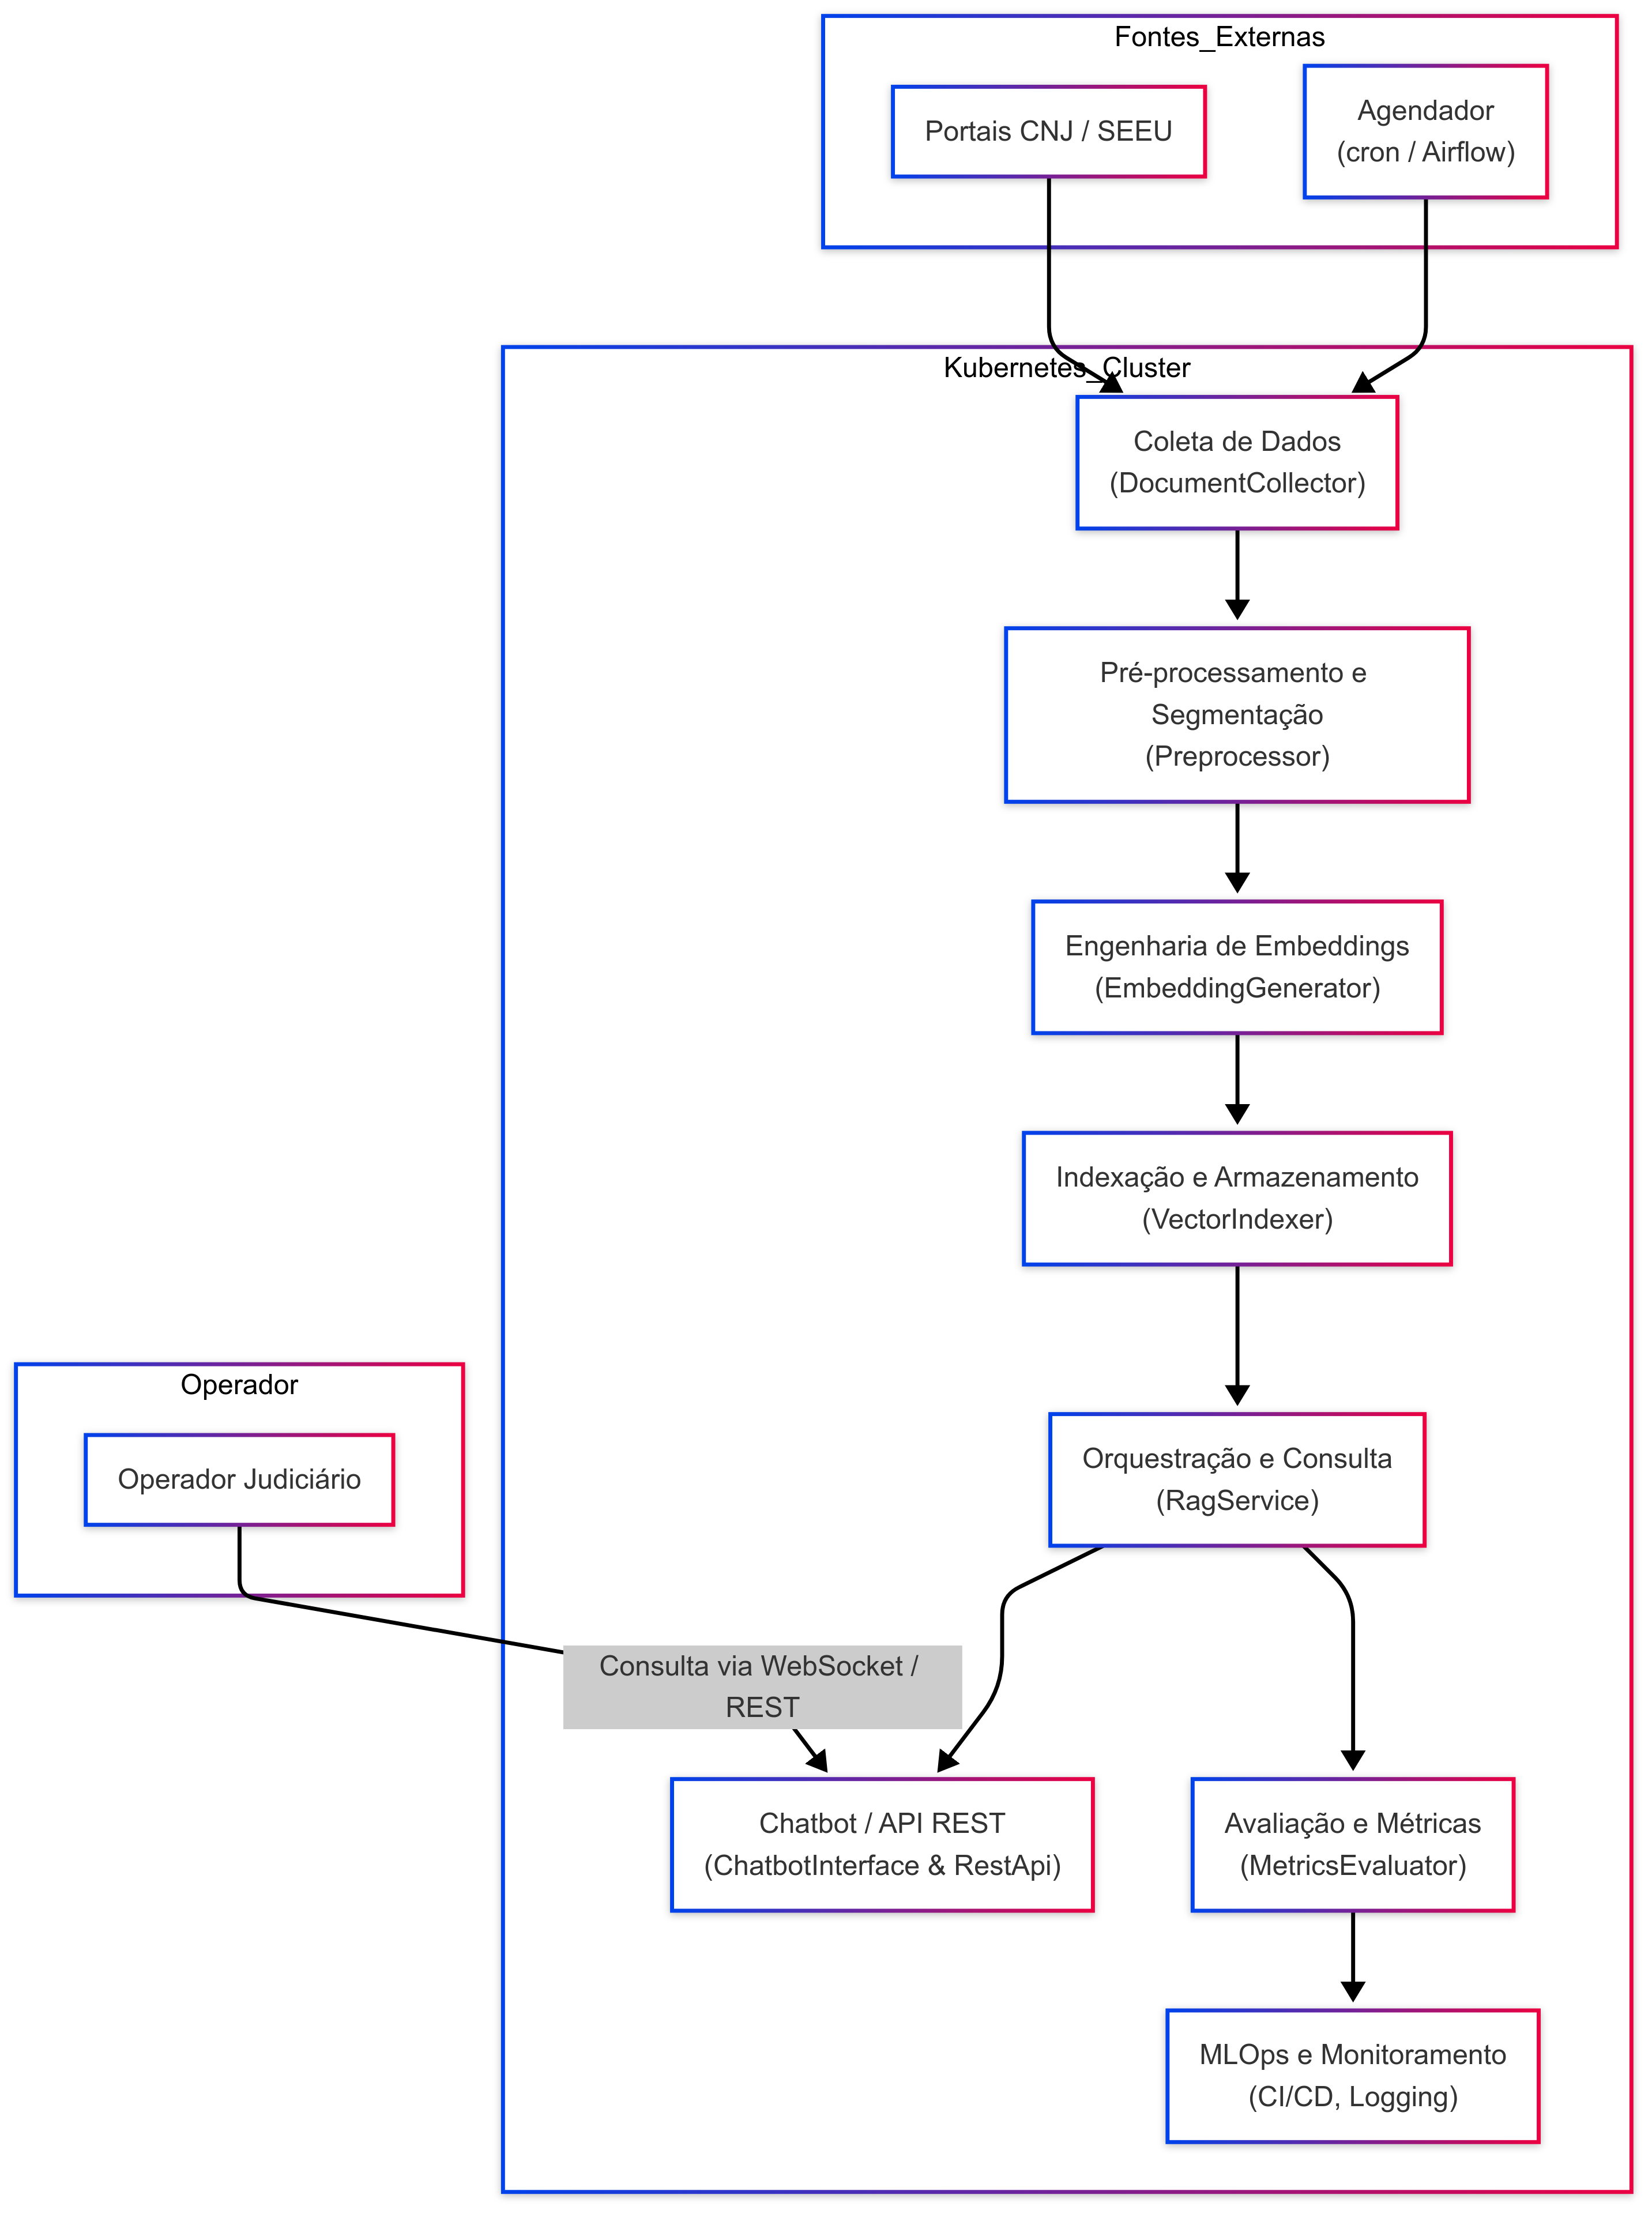
\includegraphics[width=0.8\textwidth]{04-figuras/arquitetura_pipeline.png}
  \caption{Arquitetura geral da pipeline RAG.}
  \label{fig:arquitetura_pipeline}
\end{figure}

% 4.2 Diagrama de Caso de Uso
\section{Diagrama de Caso de Uso}
\label{sec:diagrama-caso-uso}

\begin{figure}[H]
  \centering
  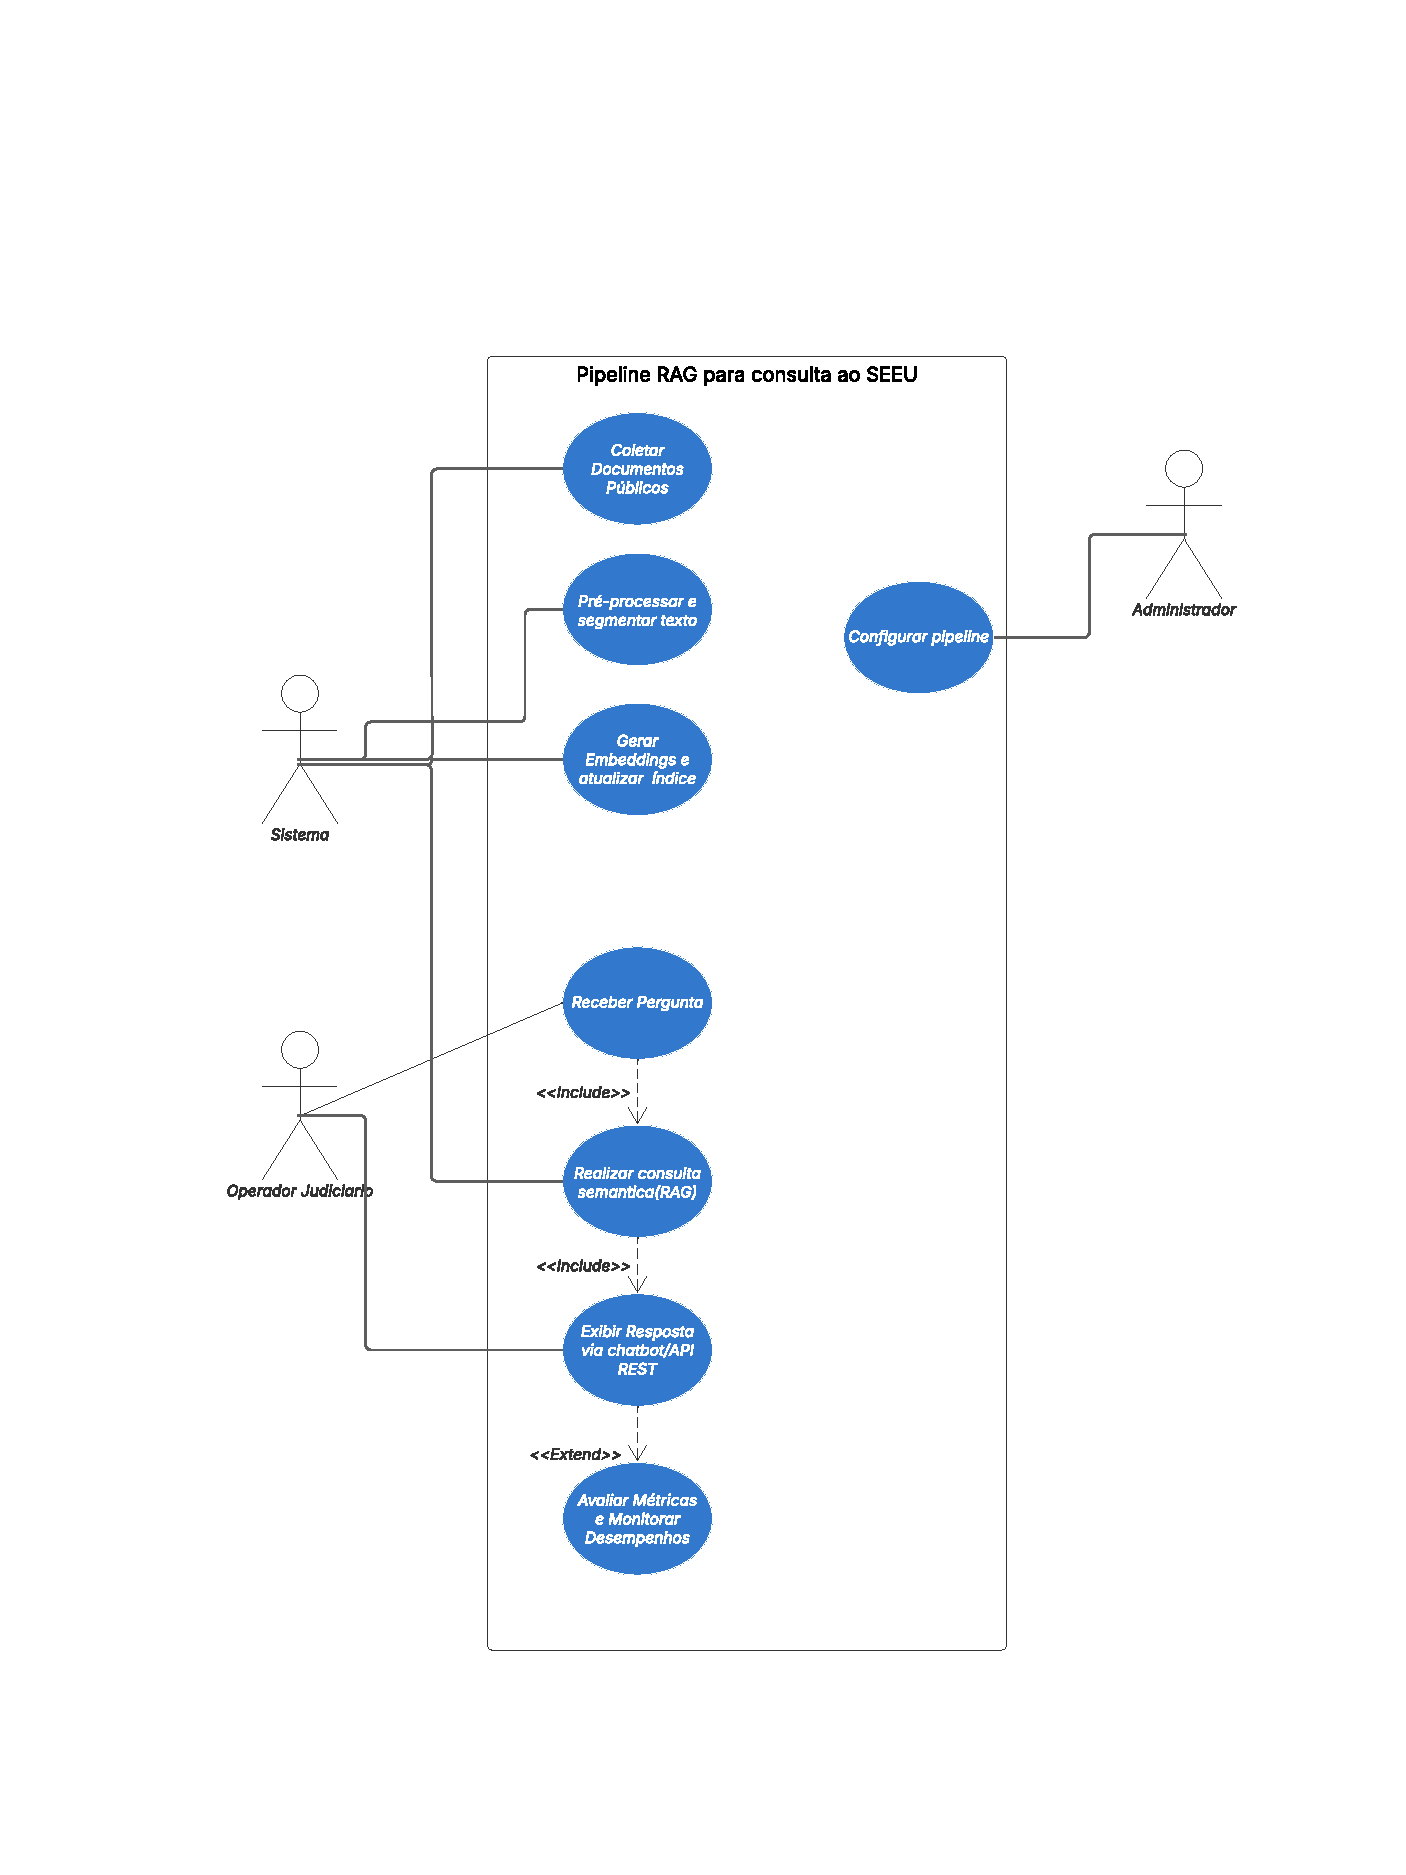
\includegraphics[width=0.9\textwidth]{04-figuras/diagrama_em_branco.pdf}
  \caption{Diagrama de Caso de Uso da Pipeline RAG para consulta ao SEEU}
  \label{fig:diagrama-rag-seeu}
\end{figure}

\noindent
O diagrama da Figura~\ref{fig:diagrama-rag-seeu} apresenta os atores e casos de uso principais da pipeline RAG para o SEEU:  
\begin{itemize}
  \item \textbf{Operador Judiciário}: inicia a consulta via “Receber Pergunta”.  
  \item \textbf{Administrador}: configura parâmetros da pipeline em “Configurar Pipeline”.  
  \item \textbf{Sistema}: atua como ator externo encarregado de disparar e orquestrar os processos de “Coletar Documentos Públicos”, “Pré-processar e segmentar texto”, “Gerar Embeddings e atualizar índice” e “Realizar Consulta Semântica (RAG)”.  
  \item \textbf{Include} (setas obrigatórias): indicam os casos de uso que são sempre invocados no fluxo principal.  
  \item \textbf{Extend} (setas opcionais): representam funcionalidades adicionais, como a “Avaliar Métricas e Monitorar Desempenho”, que estende o caso de uso “Exibir Resposta via chatbot/API REST”.  
\end{itemize}  


\subsection{Especificação de Casos de Uso}
\label{sec:especificacao-casos-uso}
No item anterior, foi apresentado o Diagrama de Caso de Uso do sistema. 
A seguir serão detalhados cada um dos casos de uso, explicando as suas interações 
com os atores:

% UC-01
\subsubsection{UC-01 – Receber Pergunta}
\noindent Este caso de uso detalha como o Operador Judiciário submete uma pergunta à pipeline, abrangendo validação, armazenamento e confirmação de recebimento.
\begin{table}[H]
  \centering
  \caption{Especificação do Caso de Uso UC-01 – Receber Pergunta}
  \label{tab:uc01}
  \begin{tabular}{|p{4cm}|p{11cm}|}
    \hline
    \textbf{Nome do caso de uso}    & UC-01 – Receber Pergunta \\ \hline
    \textbf{Atores Principais}      & Operador Judiciário      \\ \hline
    \textbf{Atores Secundários}     & —                        \\ \hline
    \textbf{Resumo}                 & Registrar a pergunta do Operador Judiciário para iniciar o processo de consulta. \\ \hline
    \textbf{Pré-Condições}          & Pipeline configurada pelo Administrador \\ \hline
    \textbf{Pós-Condições}          & Pergunta armazenada e pronta para processamento \\ \hline
    \multicolumn{2}{|l|}{\textbf{Fluxo Principal}} \\ \hline
    \multicolumn{2}{|p{15cm}|}{%
      \begin{enumerate}[label=\arabic*., leftmargin=*]
        \item Operador acessa a interface de consulta;
        \item Informa o texto da pergunta;
        \item Sistema valida e salva a pergunta;
        \item Sistema confirma o recebimento.
      \end{enumerate}
    } \\ \hline
    \multicolumn{2}{|l|}{\textbf{Fluxo Alternativo}} \\ \hline
    \multicolumn{2}{|p{15cm}|}{%
      \begin{enumerate}[label=\arabic* a\,.]
        \item Pergunta inválida: exibir erro e retornar ao passo 2;
      \end{enumerate}
      \begin{enumerate}[start=2, label=\arabic* a\,.]
        \item Falha na persistência: exibir erro crítico e registrar log.
      \end{enumerate}
    } \\ \hline
  \end{tabular}
\end{table}


% UC-02
\subsubsection{UC-02 – Configurar Pipeline}
\noindent Neste caso de uso, o Administrador configura parâmetros e módulos da pipeline RAG, garantindo que a coleta e indexação sejam executadas corretamente.
\begin{table}[H]
  \centering
  \caption{Especificação do Caso de Uso UC-02 – Configurar Pipeline}
  \label{tab:uc02}
  \begin{tabular}{|p{4cm}|p{11cm}|}
    \hline
    \textbf{Nome do caso de uso}    & UC-02 – Configurar Pipeline \\ \hline
    \textbf{Atores Principais}      & Administrador               \\ \hline
    \textbf{Atores Secundários}     & Sistema                     \\ \hline
    \textbf{Resumo}                 & Definir parâmetros e ativar módulos da pipeline RAG. \\ \hline
    \textbf{Pré-Condições}          & Ambiente de implantação disponível; credenciais de Administrador. \\ \hline
    \textbf{Pós-Condições}          & Pipeline pronta para execução de coleta, pré-processamento e indexação. \\ \hline
    \multicolumn{2}{|l|}{\textbf{Fluxo Principal}} \\ \hline
    \multicolumn{2}{|p{15cm}|}{%
      \begin{enumerate}[leftmargin=*]
        \item Administrador acessa painel de configuração;
        \item Define parâmetros de coleta (fontes, periodicidade);
        \item Seleciona opções de pré-processamento e indexação;
        \item Salva ajustes e ativa pipeline;
        \item Sistema confirma configuração bem-sucedida.
      \end{enumerate}
    } \\ \hline
    \multicolumn{2}{|l|}{\textbf{Fluxo Alternativo}} \\ \hline
    \multicolumn{2}{|p{15cm}|}{%
      \begin{enumerate}[label=\arabic* a\,.]
        \item Parâmetros inválidos: sistema exibe erro e não salva; retorna ao passo 2;
        \item Falha de autorização: sistema nega acesso e registra tentativa.
      \end{enumerate}
    } \\ \hline
  \end{tabular}
\end{table}

% UC-03
\subsubsection{UC-03 – Coletar Documentos Públicos}
\noindent Automação da extração e armazenamento de documentos públicos do SEEU, garantindo disponibilidade dos arquivos para processamento.
\begin{table}[H]
  \centering
  \caption{Especificação do Caso de Uso UC-03 – Coletar Documentos Públicos}
  \label{tab:uc03}
  \begin{tabular}{|p{4cm}|p{11cm}|}
    \hline
    \textbf{Nome do caso de uso}    & UC-03 – Coletar Documentos Públicos \\ \hline
    \textbf{Atores Principais}      & Sistema                              \\ \hline
    \textbf{Atores Secundários}     & Administrador                        \\ \hline
    \textbf{Resumo}                 & Extrair automaticamente arquivos PDF oficiais do SEEU. \\ \hline
    \textbf{Pré-Condições}          & Pipeline configurada; fontes de dados acessíveis. \\ \hline
    \textbf{Pós-Condições}          & Documentos salvos no repositório local. \\ \hline
    \multicolumn{2}{|l|}{\textbf{Fluxo Principal}} \\ \hline
    \multicolumn{2}{|p{15cm}|}{%
      \begin{enumerate}[leftmargin=*]
        \item Sistema inicia processo de coleta;
        \item Conecta-se aos portais do SEEU;
        \item Baixa novos arquivos PDF;
        \item Valida integridade e armazena no repositório.
      \end{enumerate}
    } \\ \hline
    \multicolumn{2}{|l|}{\textbf{Fluxo Alternativo}} \\ \hline
    \multicolumn{2}{|p{15cm}|}{%
      \begin{enumerate}[label=\arabic* a\,.]
        \item Falha de rede: sistema registra erro e reprograma nova tentativa;
        \item Documento corrompido: sistema descarta arquivo e alerta o Administrador.
      \end{enumerate}
    } \\ \hline
  \end{tabular}
\end{table}

% UC-04
\subsubsection{UC-04 – Pré-processar e Segmentar Texto}
\noindent Conversão de PDFs em texto, limpeza e divisão em “chunks” de tamanho controlado, preparando os dados para vetorização.
\begin{table}[H]
  \centering
  \caption{Especificação do Caso de Uso UC-04 – Pré-processar e Segmentar Texto}
  \label{tab:uc04}
  \begin{tabular}{|p{4cm}|p{11cm}|}
    \hline
    \textbf{Nome do caso de uso}    & UC-04 – Pré-processar e Segmentar Texto \\ \hline
    \textbf{Atores Principais}      & Sistema                                  \\ \hline
    \textbf{Atores Secundários}     & —                                        \\ \hline
    \textbf{Resumo}                 & Converter PDFs em texto, limpar e dividir em chunks. \\ \hline
    \textbf{Pré-Condições}          & Documentos PDF coletados disponíveis. \\ \hline
    \textbf{Pós-Condições}          & Texto limpo segmentado em unidades de tamanho definido. \\ \hline
    \multicolumn{2}{|l|}{\textbf{Fluxo Principal}} \\ \hline
    \multicolumn{2}{|p{15cm}|}{%
      \begin{enumerate}[leftmargin=*]
        \item Sistema extrai texto de cada PDF (OCR se necessário);
        \item Remove cabeçalhos, rodapés e formatação indesejada;
        \item Segmenta texto em chunks de 500–1000 tokens;
        \item Armazena chunks prontos para vetorização.
      \end{enumerate}
    } \\ \hline
    \multicolumn{2}{|l|}{\textbf{Fluxo Alternativo}} \\ \hline
    \multicolumn{2}{|p{15cm}|}{%
      \begin{enumerate}[label=\arabic* a\,.]
        \item Falha na extração (OCR): exclui chunk e registra alerta;
        \item Chunk fora do tamanho: ajusta limites e redivide automaticamente.
      \end{enumerate}
    } \\ \hline
  \end{tabular}
\end{table}

% UC-05
\subsubsection{UC-05 – Gerar Embeddings e Atualizar Índice}
\noindent Geração de embeddings a partir dos chunks de texto e inserção no banco vetorial, mantendo o índice sempre atualizado.
\begin{table}[H]
  \centering
  \caption{Especificação do Caso de Uso UC-05 – Gerar Embeddings e Atualizar Índice}
  \label{tab:uc05}
  \begin{tabular}{|p{4cm}|p{11cm}|}
    \hline
    \textbf{Nome do caso de uso}    & UC-05 – Gerar Embeddings e Atualizar Índice \\ \hline
    \textbf{Atores Principais}      & Sistema                                      \\ \hline
    \textbf{Atores Secundários}     & —                                            \\ \hline
    \textbf{Resumo}                 & Criar embeddings a partir dos chunks e indexá-los no banco vetorial. \\ \hline
    \textbf{Pré-Condições}          & Chunks de texto pré-processados disponíveis. \\ \hline
    \textbf{Pós-Condições}          & Índice vetorial atualizado com novos embeddings. \\ \hline
    \multicolumn{2}{|l|}{\textbf{Fluxo Principal}} \\ \hline
    \multicolumn{2}{|p{15cm}|}{%
      \begin{enumerate}[leftmargin=*]
        \item Sistema seleciona chunks não indexados;
        \item Calcula embeddings via modelo pré-treinado;
        \item Envia embeddings com metadados ao banco vetorial;
        \item Confirma inserção bem-sucedida no índice.
      \end{enumerate}
    } \\ \hline
    \multicolumn{2}{|l|}{\textbf{Fluxo Alternativo}} \\ \hline
    \multicolumn{2}{|p{15cm}|}{%
      \begin{enumerate}[label=\arabic* a\,.]
        \item Erro de modelo: registra falha e reprocessa chunk específico;
        \item Falha no banco: enfileira para nova tentativa e alerta Administrador.
      \end{enumerate}
    } \\ \hline
  \end{tabular}
\end{table}

% UC-06
\subsubsection{UC-06 – Realizar Consulta Semântica (RAG)}
\noindent Vetorização da pergunta do Operador, recuperação dos documentos mais relevantes e geração de resposta via LLM, seguida de registro de logs.
\begin{table}[H]
  \centering
  \caption{Especificação do Caso de Uso UC-06 – Realizar Consulta Semântica (RAG)}
  \label{tab:uc06}
  \begin{tabular}{|p{4cm}|p{11cm}|}
    \hline
    \textbf{Nome do caso de uso}    & UC-06 – Realizar Consulta Semântica (RAG) \\ \hline
    \textbf{Atores Principais}      & Operador Judiciário                       \\ \hline
    \textbf{Atores Secundários}     & Sistema                                   \\ \hline
    \textbf{Resumo}                 & Vetorizar pergunta, recuperar documentos e gerar resposta via LLM. \\ \hline
    \textbf{Pré-Condições}          & Índice vetorial disponível; pergunta recebida. \\ \hline
    \textbf{Pós-Condições}          & Resposta gerada e pronta para exibição. \\ \hline
    \multicolumn{2}{|l|}{\textbf{Fluxo Principal}} \\ \hline
    \multicolumn{2}{|p{15cm}|}{%
      \begin{enumerate}[leftmargin=*]
        \item Operador submete pergunta armazenada;
        \item Sistema vetoriza a pergunta;
        \item Recupera top-k chunks semânticos do índice;
        \item Concatena evidências ao prompt do LLM;
        \item Gera e formata resposta natural;
        \item Armazena log da consulta e resposta.
      \end{enumerate}
    } \\ \hline
    \multicolumn{2}{|l|}{\textbf{Fluxo Alternativo}} \\ \hline
    \multicolumn{2}{|p{15cm}|}{%
      \begin{enumerate}[label=\arabic* a\,.]
        \item Índice indisponível: exibe mensagem de erro e sugere reintentar;
        \item LLM sem resposta: exibe fallback com fonte oficial.
      \end{enumerate}
    } \\ \hline
  \end{tabular}
\end{table}

% UC-07
\subsubsection{UC-07 – Exibir Resposta via Chatbot/API REST}
\noindent Formatação e envio da resposta ao Operador por meio de interface conversacional ou endpoint REST, com confirmação e registro de entrega.
\begin{table}[H]
  \centering
  \caption{Especificação do Caso de Uso UC-07 – Exibir Resposta via Chatbot/API REST}
  \label{tab:uc07}
  \begin{tabular}{|p{4cm}|p{11cm}|}
    \hline
    \textbf{Nome do caso de uso}    & UC-07 – Exibir Resposta via Chatbot/API REST \\ \hline
    \textbf{Atores Principais}      & Operador Judiciário                          \\ \hline
    \textbf{Atores Secundários}     & Sistema                                      \\ \hline
    \textbf{Resumo}                 & Enviar resposta ao Operador por meio de interface conversacional ou API. \\ \hline
    \textbf{Pré-Condições}          & Resposta gerada e disponível no sistema. \\ \hline
    \textbf{Pós-Condições}          & Operador recebe e visualiza resposta; log de entrega registrado. \\ \hline
    \multicolumn{2}{|l|}{\textbf{Fluxo Principal}} \\ \hline
    \multicolumn{2}{|p{15cm}|}{%
      \begin{enumerate}[leftmargin=*]
        \item Sistema formata resposta para chatbot e JSON de API;
        \item Envia mensagem pelo canal WebSocket ou endpoint REST;
        \item Recebe confirmação de entrega;
        \item Armazena status de entrega.
      \end{enumerate}
    } \\ \hline
    \multicolumn{2}{|l|}{\textbf{Fluxo Alternativo}} \\ \hline
    \multicolumn{2}{|p{15cm}|}{%
      \begin{enumerate}[label=\arabic* a\,.]
        \item Falha no canal: tenta rota alternativa (API ↔ chatbot);
        \item Erro de formatação: registra exceção e notifica Administrador.
      \end{enumerate}
    } \\ \hline
  \end{tabular}
\end{table}

% UC-08
\subsubsection{UC-08 – Avaliar Métricas e Monitorar Desempenhos}
\noindent Cálculo de métricas (precisão, recall, F1, latência) com base em logs de consulta, atualização do dashboard e acionamento de alertas quando necessário
\begin{table}[H]
  \centering
  \caption{Especificação do Caso de Uso UC-08 – Avaliar Métricas e Monitorar Desempenhos}
  \label{tab:uc08}
  \begin{tabular}{|p{4cm}|p{11cm}|}
    \hline
    \textbf{Nome do caso de uso}    & UC-08 – Avaliar Métricas e Monitorar Desempenhos \\ \hline
    \textbf{Atores Principais}      & Sistema                                           \\ \hline
    \textbf{Atores Secundários}     & Administrador                                     \\ \hline
    \textbf{Resumo}                 & Calcular precisão, recall, F1 e acompanhar latência. \\ \hline
    \textbf{Pré-Condições}          & Logs de consultas e respostas disponíveis. \\ \hline
    \textbf{Pós-Condições}          & Dashboard de métricas atualizado; alertas acionados se limites ultrapassados. \\ \hline
    \multicolumn{2}{|l|}{\textbf{Fluxo Principal}} \\ \hline
    \multicolumn{2}{|p{15cm}|}{%
      \begin{enumerate}[leftmargin=*]
        \item Sistema agrega dados de logs de consulta;
        \item Calcula métricas (precisão, recall, F1, latência);
        \item Atualiza painel de monitoramento;
        \item Se métricas fora do padrão, gera alerta ao Administrador.
      \end{enumerate}
    } \\ \hline
    \multicolumn{2}{|l|}{\textbf{Fluxo Alternativo}} \\ \hline
    \multicolumn{2}{|p{15cm}|}{%
      \begin{enumerate}[label=\arabic* a\,.]
        \item Dados incompletos: sinaliza alerta de qualidade de log e pausa processamento;
        \item Falha no cálculo: registra erro e envia notificação emergencial.
      \end{enumerate}
    } \\ \hline
  \end{tabular}
\end{table}

% 4.3 Diagrama de Classe
\section{Diagrama de Classes}
\label{sec:diagrama-de-classes}
\noindent No item anterior, foram apresentadas as Descrições dos Casos de Uso 
sistema. A seguir será apresentado o Diagrama de Classe contendo todos os 
atributos, métodos e relacionamentos

\begin{figure}[H]
  \centering
  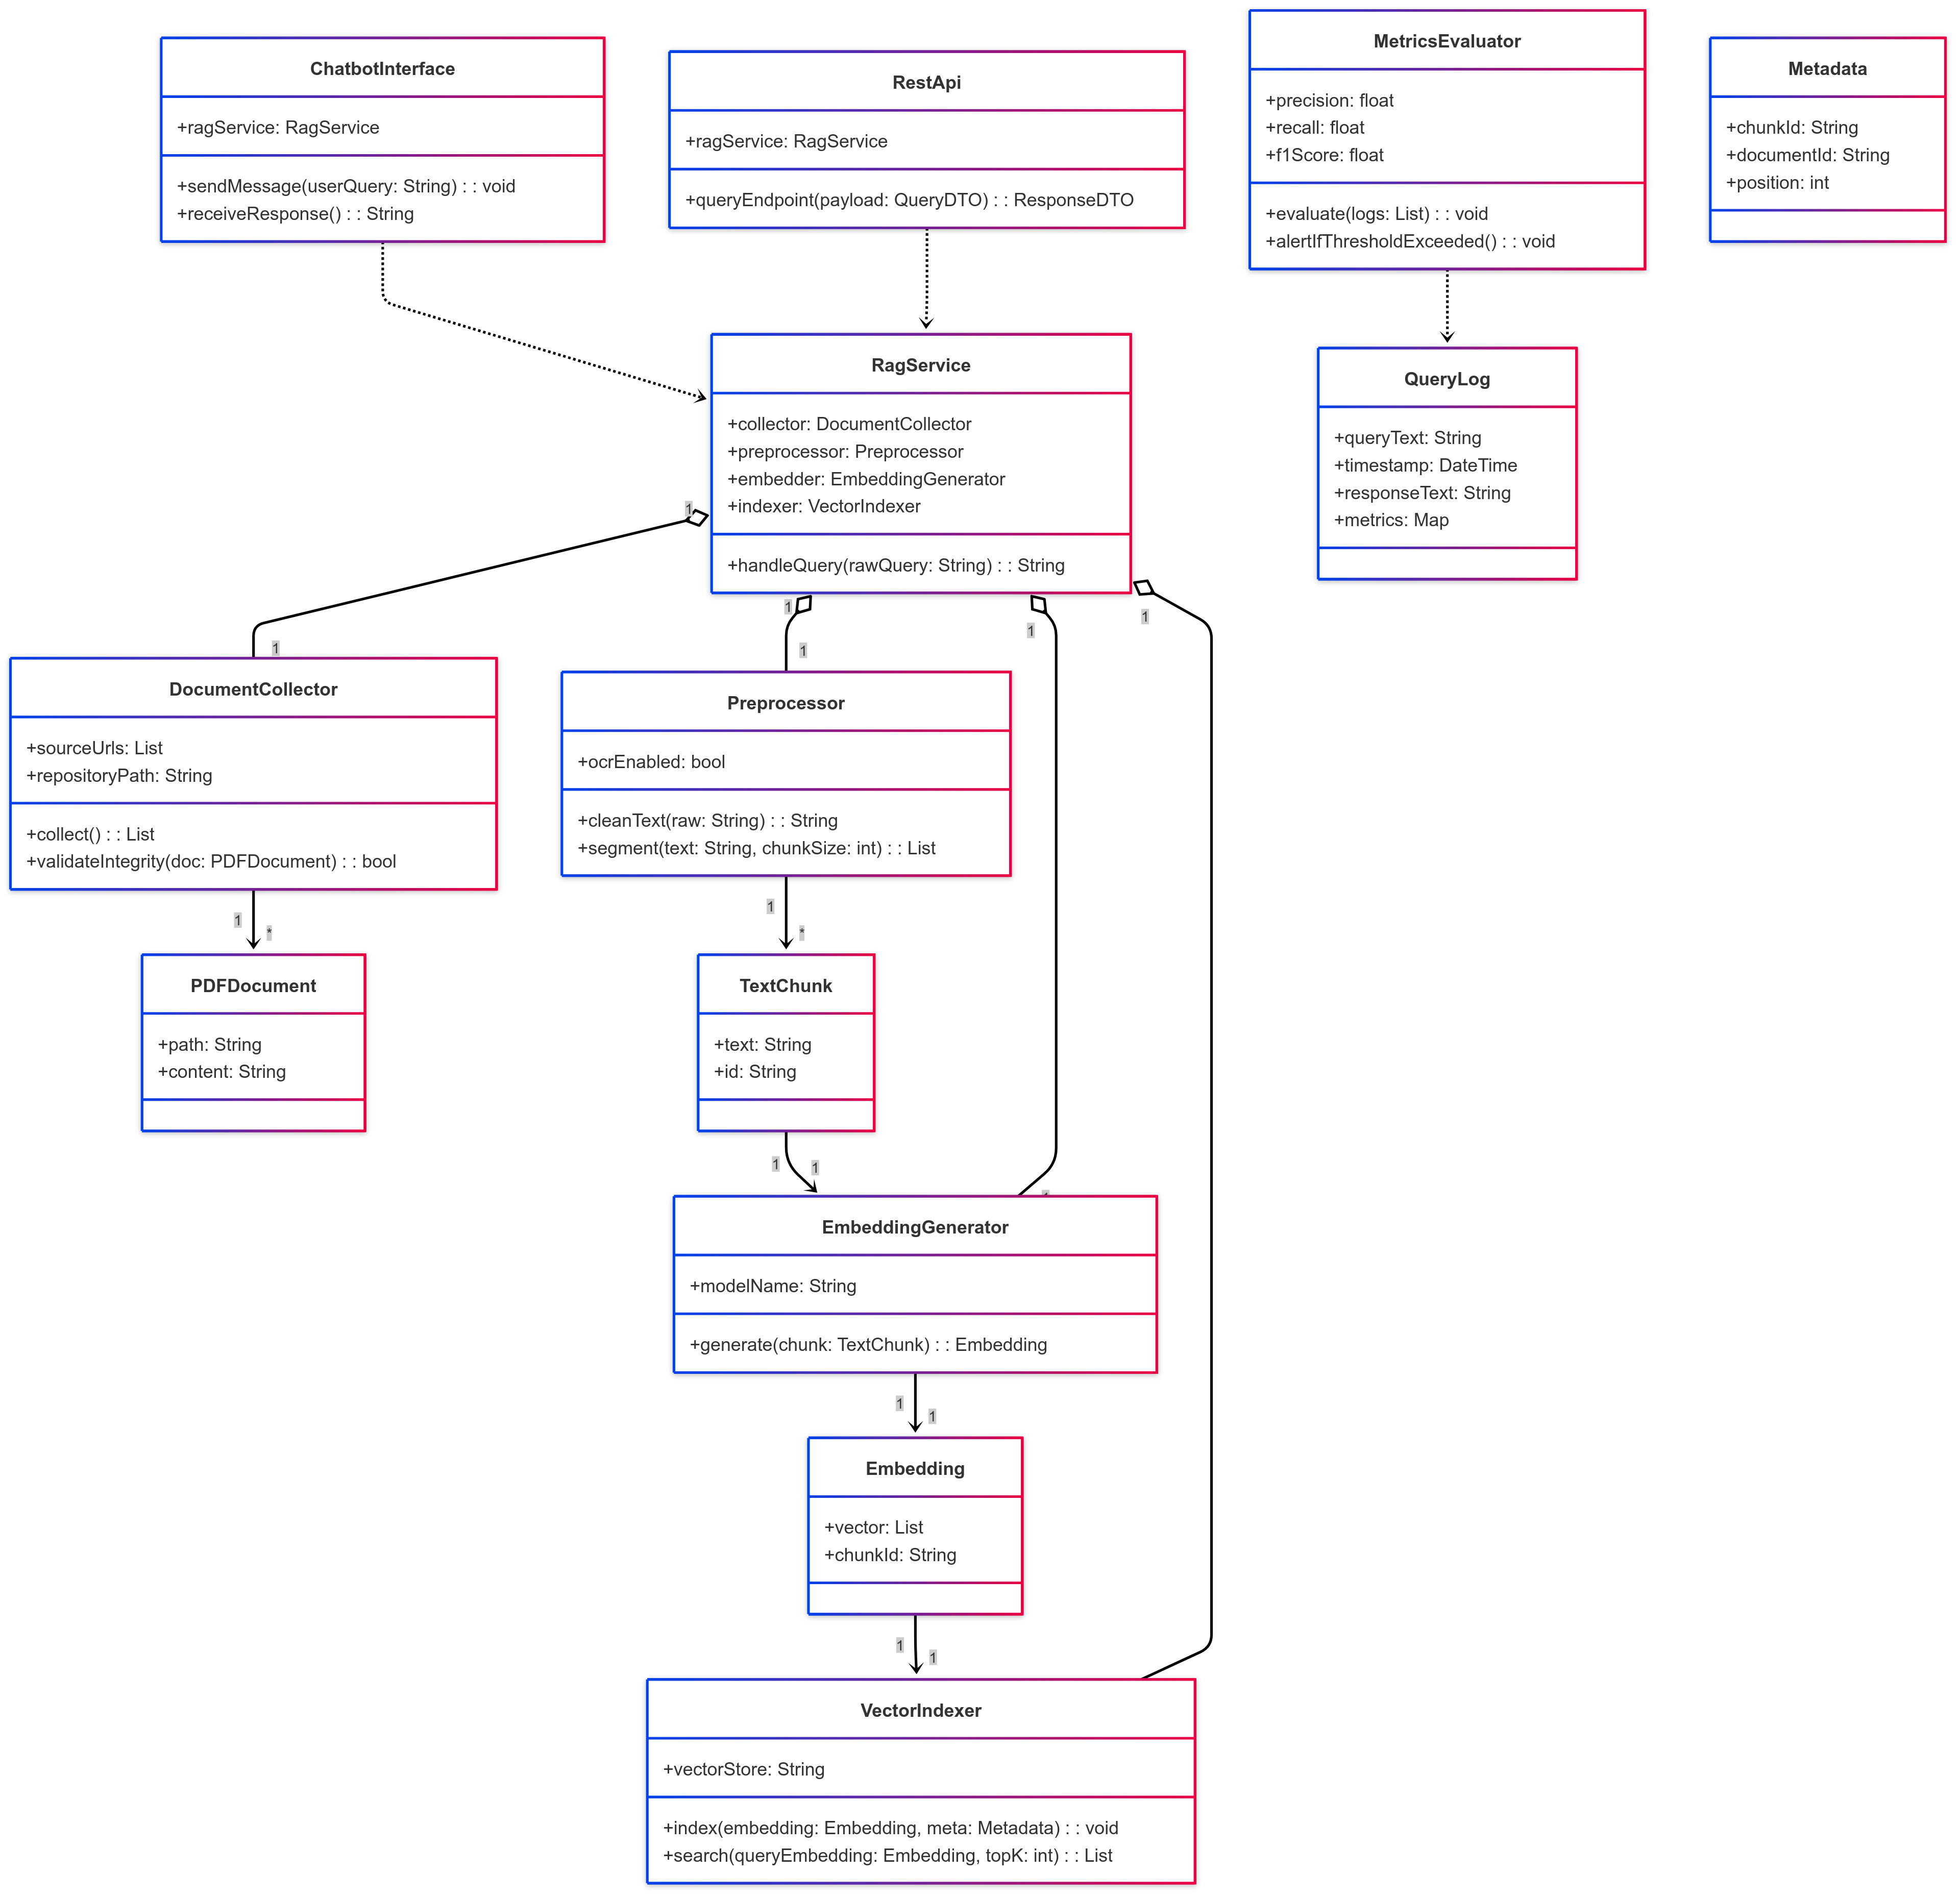
\includegraphics[width=0.9\textwidth]{04-figuras/diagrama_de_classe.png}
  \caption{Diagrama de Caso de Uso da Pipeline RAG para consulta ao SEEU}
  \label{fig:diagrama-rag-seeu}
\end{figure}

\noindent A Figura 3 apresenta o Diagrama de Classe, mostrando os atributos, 
métodos e relacionamentos das classes no sistema 

% Dicionário de Dados: PDFDocument
\begin{table}[H]
  \centering
  \caption{Dicionário de Dados da entidade \texttt{PDFDocument}}
  \label{tab:dd_pdfdocument}
  \begin{tabular}{|p{3cm}|p{4cm}|p{8cm}|}
    \hline
    \textbf{Campo} & \textbf{Tipo} & \textbf{Descrição} \\ \hline
    \texttt{path}     & \texttt{String} & Caminho completo no sistema de arquivos onde o PDF foi salvo. \\ \hline
    \texttt{content}  & \texttt{String} & Texto bruto extraído do PDF (após OCR, se aplicável). \\ \hline
  \end{tabular}
\end{table}

% Dicionário de Dados: TextChunk
\begin{table}[H]
  \centering
  \caption{Dicionário de Dados da entidade \texttt{TextChunk}}
  \label{tab:dd_textchunk}
  \begin{tabular}{|p{3cm}|p{4cm}|p{8cm}|}
    \hline
    \textbf{Campo} & \textbf{Tipo} & \textbf{Descrição} \\ \hline
    \texttt{id}    & \texttt{String} & Identificador único do fragmento de texto. \\ \hline
    \texttt{text}  & \texttt{String} & Conteúdo textual do chunk, tipicamente 500–1000 tokens. \\ \hline
  \end{tabular}
\end{table}

% Dicionário de Dados: Embedding
\begin{table}[H]
  \centering
  \caption{Dicionário de Dados da entidade \texttt{Embedding}}
  \label{tab:dd_embedding}
  \begin{tabular}{|p{3cm}|p{4cm}|p{8cm}|}
    \hline
    \textbf{Campo}     & \textbf{Tipo}            & \textbf{Descrição} \\ \hline
    \texttt{vector}     & \texttt{List<float>}     & Lista de valores numéricos que compõem o embedding semântico. \\ \hline
    \texttt{chunkId}    & \texttt{String}          & Chave estrangeira para o \texttt{TextChunk} de origem. \\ \hline
  \end{tabular}
\end{table}

% Dicionário de Dados: Metadata
\begin{table}[H]
  \centering
  \caption{Dicionário de Dados da entidade \texttt{Metadata}}
  \label{tab:dd_metadata}
  \begin{tabular}{|p{3cm}|p{4cm}|p{8cm}|}
    \hline
    \textbf{Campo}       & \textbf{Tipo}   & \textbf{Descrição} \\ \hline
    \texttt{chunkId}      & \texttt{String} & Referência ao fragmento de texto indexado. \\ \hline
    \texttt{documentId}   & \texttt{String} & Identificador do documento PDF de origem. \\ \hline
    \texttt{position}     & \texttt{int}    & Posição do chunk dentro do documento (ordem sequencial). \\ \hline
  \end{tabular}
\end{table}

% Dicionário de Dados: QueryLog
\begin{table}[H]
  \centering
  \caption{Dicionário de Dados da entidade \texttt{QueryLog}}
  \label{tab:dd_querylog}
  \begin{tabular}{|p{3cm}|p{4cm}|p{8cm}|}
    \hline
    \textbf{Campo}       & \textbf{Tipo}         & \textbf{Descrição} \\ \hline
    \texttt{queryText}    & \texttt{String}       & Texto original da pergunta submetida pelo operador. \\ \hline
    \texttt{timestamp}    & \texttt{DateTime}     & Data e hora em que a consulta foi processada. \\ \hline
    \texttt{responseText} & \texttt{String}       & Resposta gerada pela LLM após RAG. \\ \hline
    \texttt{metrics}      & \texttt{Map<String,float>} & Mapa contendo valores de precisão, recall, F1 e latência para aquela consulta. \\ \hline
  \end{tabular}
\end{table}

% 4.4 Protótipos
\section{Protótipos}
\label{sec:prototipos}
\noindent Abaixo serão apresentados os protótipos e o funcionamento do sistema. Estes protótipos ilustram as principais telas e funcionalidades do sistema, demonstrando como os usuários podem interagir com o sistema.


%%%%%%%%%%%%%%%%%%%%%%%%%%%%%%%%%%%%%%%%%%%%%%%%%%%%%%%%%%%%%%%%%%%%%%%%%%%%%%%
% CAPÍTULO 5 – RESULTADOS ESPERADOS
%%%%%%%%%%%%%%%%%%%%%%%%%%%%%%%%%%%%%%%%%%%%%%%%%%%%%%%%%%%%%%%%%%%%%%%%%%%%%%%

\chapter{Resultados Esperados}
\label{chap:resultados}

Este capítulo descreve, de forma detalhada, os resultados que se almeja alcançar com a execução do presente Trabalho de Conclusão de Curso (TCC). Tais resultados derivam dos objetivos estabelecidos no Capítulo~\ref{sec:objetivos} e da metodologia apresentada no Capítulo~\ref{chap:metodologia}, respeitando as normas da Associação Brasileira de Normas Técnicas -- ABNT (NBR 14724:2011) para trabalhos acadêmicos.

\section{Implementação de uma pipeline RAG funcional}
Espera-se disponibilizar uma pipeline de RAG plenamente operacional, capaz de integrar um modelo de LLM a um índice vetorial que contenha os documentos públicos do SEEU. A solução deverá oferecer uma interface conversacional (chatbot) em língua portuguesa, além de uma API REST para consumo externo, permitindo consultas em linguagem natural e retornando respostas fundamentadas nos documentos originais.

\section{Ganho de eficiência na recuperação de informações}
A implementação proposta deverá reduzir o tempo médio despendido pelos operadores do Direito para localizar e consolidar informações no SEEU, quando comparado ao processo manual atualmente utilizado. Tal meta será verificada por meio de ensaios controlados que mensurem o tempo de resposta antes e depois da adoção da ferramenta. Objetiva-se uma redução de pelo menos 80\% no tempo de busca.

\section{Melhoria da qualidade das respostas}
Pretende-se atingir índices de precisão iguais ou superiores a 0,85, \emph{recall} mínimo de 0,80 e \emph{F\textsubscript{1}-score} não inferior a 0,82 na recuperação dos trechos mais relevantes, conforme protocolo de avaliação descrito na Seção~6.1. Esses valores garantirão a confiabilidade do sistema e a relevância das informações apresentadas ao usuário.

\section{Redução de alucinações do modelo}
A integração entre o LLM e o mecanismo de recuperação semântica deverá limitar a incidência de respostas não fundamentadas (alucinações) a, no máximo, 5\% do total de interações. Essa meta será monitorada por meio de amostragem estatística das conversas, com posterior verificação manual do conteúdo gerado.

\section{Escalabilidade e portabilidade comprovadas}
A solução será entregue em contêineres Docker, orquestrados via Kubernetes, garantindo a portabilidade entre ambientes e a escalabilidade horizontal necessária para lidar com picos de demanda, sem que a latência média de recuperação ultrapasse 1 s para consultas padrão.

\section{Integração institucional e impacto social}
Almeja-se que o protótipo desenvolvido se alinhe às iniciativas de transformação digital do Conselho Nacional de Justiça (Programa Justiça 4.0) e aos Objetivos de Desenvolvimento Sustentável nº 16 da Organização das Nações Unidas, contribuindo para a transparência e o acesso à justiça de populações vulnerabilizadas.

\section{Base para melhoria contínua}
Será implementado um mecanismo de \emph{feedback loop} que registre as interações dos usuários e permita o re-treinamento periódico do modelo de linguagem, assegurando a evolução constante do sistema e a adaptação às mudanças normativas ou procedimentais.

\section{Documentação técnica completa}
Serão entregues: código-fonte comentado, arquivos \texttt{Dockerfile}, manual do desenvolvedor, manual do usuário final e documentação da API. Essa documentação facilitará a reprodutibilidade acadêmica e a eventual adoção da solução por outros órgãos do Judiciário.

\section{Mitigação de riscos operacionais}
O projeto contemplará um plano de mitigação de riscos que inclua atualização contínua de dependências \emph{open source}, testes automatizados de regressão e políticas de segurança da informação, garantindo a confiabilidade e a sustentabilidade da aplicação em produção.

A consecução dos resultados elencados neste capítulo demonstrará a viabilidade técnica e o impacto prático da aplicação de técnicas de RAG na execução penal brasileira, servindo de base para futuras pesquisas e para possíveis expansões em âmbito nacional.

%%%%%%%%%%%%%%%%%%%%%%%%%%%%%%%%%%%%%%%%%%%%%%%%%%%%%%%%%%%%%%%%%%%%%%%%%%%%%%%
% CAPÍTULO 6 – CONCLUSÕES
%%%%%%%%%%%%%%%%%%%%%%%%%%%%%%%%%%%%%%%%%%%%%%%%%%%%%%%%%%%%%%%%%%%%%%%%%%%%%%%

\chapter{Conclusões}
\label{chap:conclusoes}

A pipeline proposta demonstra a viabilidade de aplicar RAG ao SEEU, alinhando-se a iniciativas de Justiça 4.0 e ODS 16. Com redução de tempo e maior precisão, espera-se uma execução penal mais transparente e eficiente. Trabalhos futuros podem expandir o escopo para outros domínios jurídicos e refinar embeddings em português jurídico.
\include{02-elementos-textuais/fundamentacao}
\include{02-elementos-textuais/tecnologias}
\include{02-elementos-textuais/metodologia}
\include{02-elementos-textuais/resultados}

% ====================================================
% Elementos pós-textuais
% ====================================================
\postextual
\bibliography{referencias}

\end{document}